\begin{figure}[!htb]
\centering
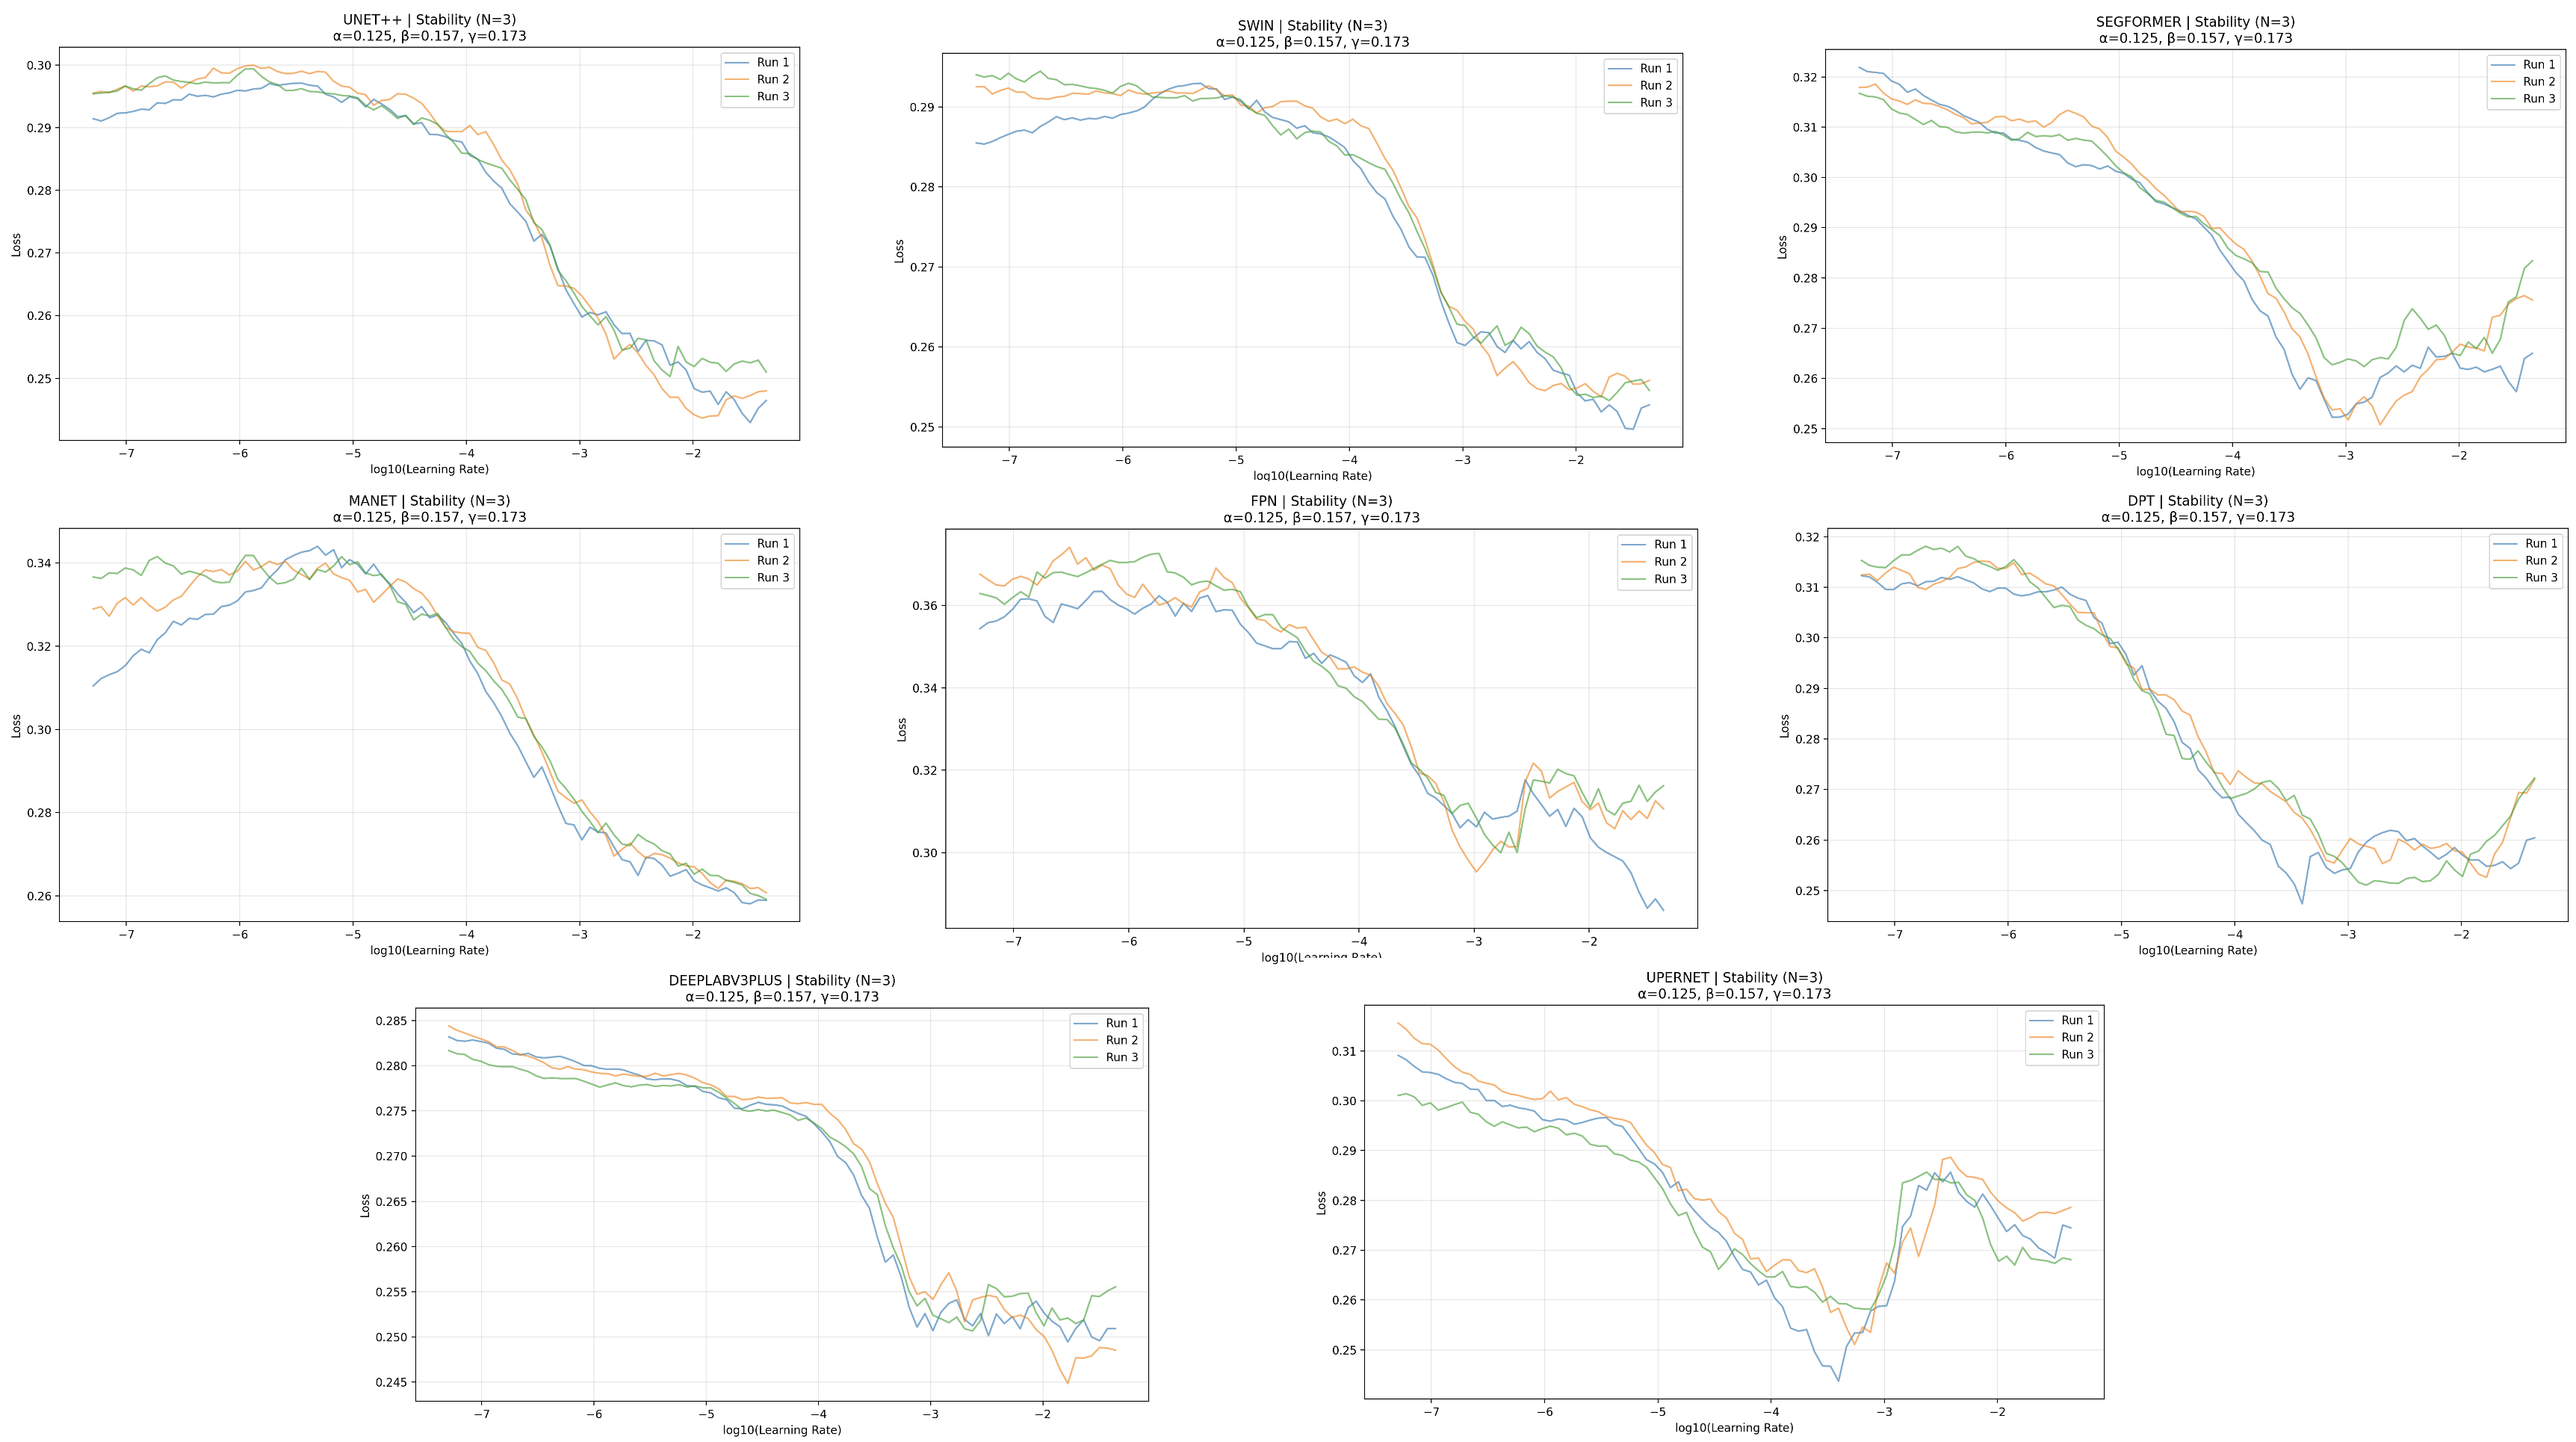
\includegraphics[width=\textwidth]{figuras/DIAGSET_NOT_NORMALIZED_LR.png}

\caption[Curvas de busca de taxa de aprendizado para DIAGSET sem normalização]{
Curvas de busca de taxa de aprendizado para os modelos treinados no conjunto
DIAGSET sem normalização de cor. Cada subgráfico apresenta a evolução da função
de perda em função de $\log_{10}$ da taxa de aprendizado para uma arquitetura
avaliada, com três execuções independentes. As curvas foram utilizadas para
identificar regiões de queda estável da perda e selecionar taxas de aprendizado
candidatas para o treinamento final.
}
\label{fig:results_diagset-lr-curves-not-normalized}
\end{figure}

\begin{table}[!htb]
\centering
\caption{Taxas de aprendizado selecionadas para o treinamento final no DIAGSET sem normalização de cor.}
\label{tab:results_diagset-learning-rates-not-normalized}
\begin{tabular}{lr}
\toprule
Arquitetura & LR ($10^{-3}$) \\
\midrule
DEEPLABV3PLUS & 0.1 \\
DPT & 0.1 \\
FPN & 0.3 \\
MANET & 1.0 \\
SEGFORMER & 0.1 \\
SWIN & 0.1 \\
UNET++ & 1.0 \\
UPERNET & 0.06 \\
\bottomrule
\end{tabular}
\end{table}